\documentclass[usletter]{article}
\usepackage{graphicx}
\usepackage{amsfonts}
\usepackage{amsthm}
\usepackage{amsmath}
\usepackage{scribe}
\usepackage[margin=1.5in]{geometry}
\usepackage{algorithm}
\usepackage{algorithmicx}
\usepackage[noend]{algpseudocode}

\begin{document}

\makeheader{Minsheng Zhang}                              % your name
           {February 15, 2015}                          % lecture date
           {6}                                       % lecture number
           {Transformation  and DP}  % lecture title

\noindent
During this, we continue to learn about the algorithm of max flow and some transformation problem of it. Then we discuss the independent set and start to talk about NP problem.  

\section{Bipartite matching}
First, we solve Bipartite matching using two different methods by solving max flow and linear programming.

A Bipartite Graph G = (V, E) is a graph in which the vertex set V can be divided into two disjoint subsets X and Y such that every edge e $\subset$ E has one end point in X and the other end point in Y. A matching M is a subset of edges such that each node in V appears in at most one edge in M.

First, we solve maximum BM problem by transfroming it to max flow as shown in  Figure~\ref{fig:bm-mf}
\begin{enumerate}
	\item Add a source node and add edges from source node to all the nodes in X.\item Add a sink node and add edges from nodes in Y to sink node.
	\item Use Ford-Fulkerson algorithm to find the maximum flow in the new flow network. The maximum flow is the maximum BM.
\end{enumerate}

We can observe that: (which can be used to conclude that bm can be reduced to mf.)
\begin{enumerate}
	\item There is no node in X which has more than one outgoing edge where there is a flow.
	\item There is no node in Y which has more than one incoming edge where there is a flow.
	\item  The number of edges between X and Y which carry flow is k
\end{enumerate}

\begin{figure}[bht]
\begin{center}
     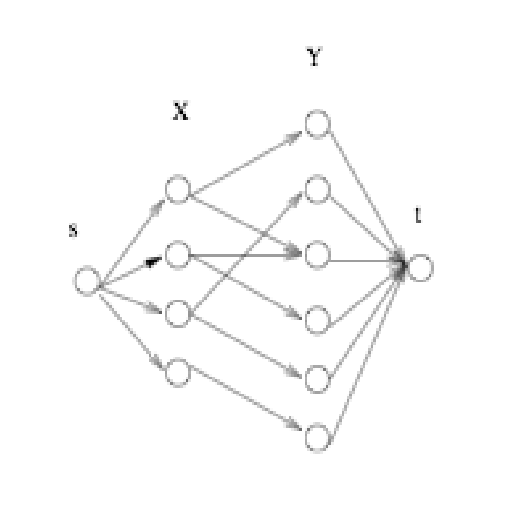
\includegraphics[width=3.0in]{figures/bm-mf}
\caption{\label{fig:bm-mf}Bipartite matching and max flow}
\end{center}
\end{figure}

Still, we can solve this problem by linear programming as shown in Figure~\ref{fig:bm-lp} (note here should be ILP).
\begin{enumerate}
	\item maximum the sum of all the edges.(The value of the edges can be 1 or 0)
	\item for all the vertices. the number of connected edges <= 1
\end{enumerate}

\section{Independent Set}
We continue talking about Independent set problems. In graph theory, an independent set or stable set is a set of vertices in a graph, no two of which are adjacent. We can have a decision, search and optimization questions about independent set for a given Graph G and k vetices.

\begin{enumerate}
	\item Decision: is there an IS with k vertices.
	\item Search: find an IS with K vertices.
	\item Optimization: Find the largest IS.
\end{enumerate}

Here we introduce reduction here which means by solving problem A we can solve problem B as shown in Figure~\ref{fig:relation}. Use reduction or transformation, we can easily solve search version of IS by solving the decision version. 

\begin{figure}[bht]
\begin{center}
     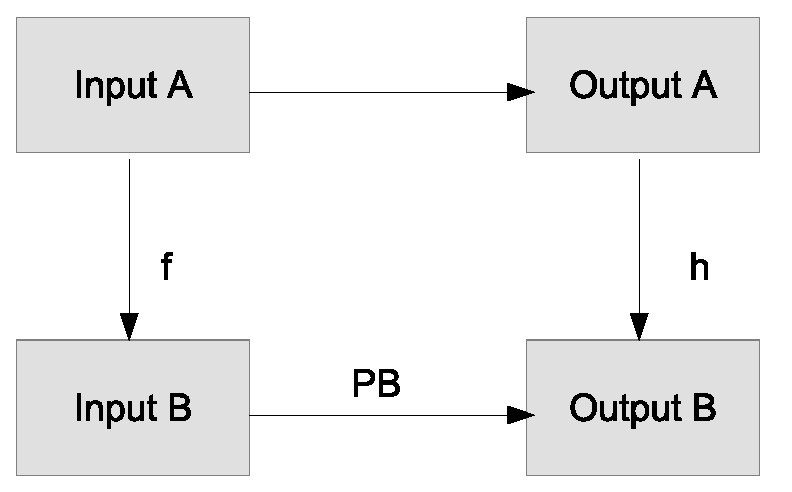
\includegraphics[width=3.0in]{figures/reduction}
\caption{\label{fig:relation}Relation}
\end{center}
\end{figure}

\begin{algorithm}
\caption{ISS}
\begin{algorithmic}[1]
\Procedure{ISS}{G, k}
\For{\texttt{i = 1 to n}}
	\State $G' = G - {v} - N{v}$
	\If {$\Call {ISD}{G', k-1}$}
		\State \Return $v_{i} \cup \Call {ISS}{G', k-1}$
	\EndIf
\EndFor
\State \Return $nil$
\EndProcedure
\end{algorithmic}
\end{algorithm}


Also, we can solve the Optimization version of IS by solving the integer linear programming problem as shown in Figure~\ref{fig:optimization}

For any $v \in V$ make a variable $X_v$ ∈ {0, 1}
\begin{enumerate}
	\item $X_v$ = 0 when v is not in the MIS.
	\item $X_v$ = 1 which v is in the MIS.
\end{enumerate}

Then for the LIP we have:
\begin{enumerate}
	\item Maximize $X_v$ where $v \in V$
	\item for each edge (u,v), $X_u + X_v <= 1$
\end{enumerate}

\begin{figure}[bht]
\begin{center}
     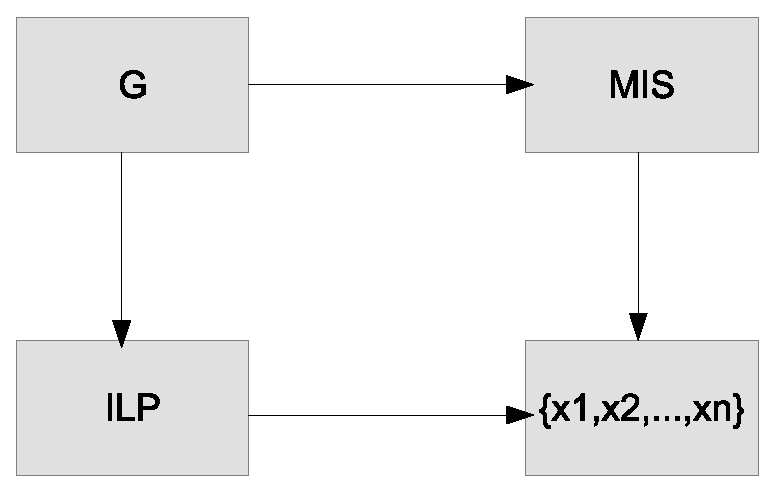
\includegraphics[width=3.0in]{figures/optimization}
\caption{\label{fig:optimization}MIS and ILP}
\end{center}
\end{figure}

\section{Circuit evaluation}
Given a set of or, not and gates and one of the gates is designated as the output as shown in Figure~\ref{fig:circuit-evaluation}

\begin{figure}[bht]
\begin{center}
     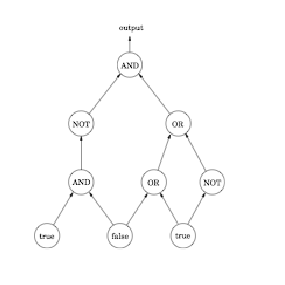
\includegraphics[width=3.0in]{figures/circuit-evaluation}
\caption{\label{fig:circuit-evaluation}circuit evaluation example}
\end{center}
\end{figure}

The CIRCUIT Evaluation problem is the following: when the laws of Boolean logic are applied to the gates in topological order, does the output evaluate to true?

We can solve the CE problem by solving the LP problem as shown in Figure~\ref{fig:CE-LP}.

The transformation is: ($x_g is the output, x_h and x_h' are the intput$)
\begin{enumerate} 
	\item 	Not gate: $x_{g}$ = 1 - $x_{h}$ 
	\item Or gate: $x_{g} \ge x_{h}; x_{g} \ge x_{h'}; x_{g} \le x_{h} + x_{h'}$.
	\item And gate: $x_{g} \le x_{h}; x_{g} \le x_{h'}; x_{g} \ge x_{h} + x_{h'} - 1$.
\end{enumerate}

These constraints force all the gates to take on exactly the right values—0 for false, and 1 for true. And we do not need to get maximum or minimum output, what we need is to just get the answer from the ouput gate.

\begin{figure}[bht]
\begin{center}
     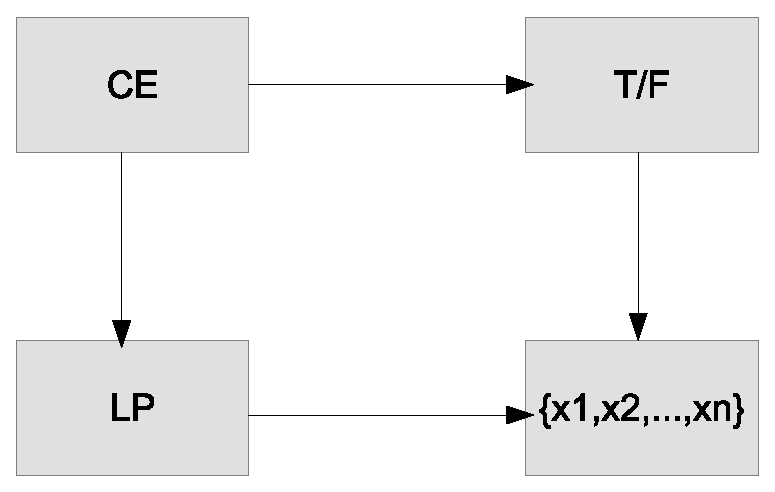
\includegraphics[width=3.0in]{figures/CE-LP}
\caption{\label{fig:CE-LP}circuit evaluation and linear programming}
\end{center}
\end{figure}

\section{NP problem}
First we talk about the definition of P, NP and NPC. Then we have some examples of these problems and discuss the relation ship of them.
P: seach problems solvable in polynomial time. $(O(n^k))$
NP: seach problems whose solutions can be verified in polynomial time.
sorting $\in$ P, sorting $\in$ NP
IS $\in$ NP, VC $\in$ NP
We know that P $\subset$ NP, but we are not sure P $\subseteq$ NP, as currectly we do not know whether P is equal to NP or not.

Then we start to learn NP complete problems which is a subset of NP. We have the definitions:

If A $\in$ NPC, then
\begin{enumerate}
	\item A $\in$ NP.
	\item if B $\in$ NPC, then B $\rightarrow$ A in $(O(n^k))$.
\end{enumerate}

So we can make a conclude that if A $\in$ NPC and A is solvable in polynomial time which means A $\in$ P, then $P=NP$

The first NPC problem is SAT problem. (2SAT is not a NPC problem)

\begin{theorem}
$Cook's$ theorem:
If C $\in$ NP and SAT $\rightarrow$ C in $(O(n^k))$, then C $\in$ NPC
\end{theorem}

We can pick any B $\in$ NP,  B $\rightarrow$ SAT $\rightarrow$ C. And we can see the reulations of B, SAT and C in Figure~\ref{fig:relation-npc}

\begin{figure}[bht]
\begin{center}
     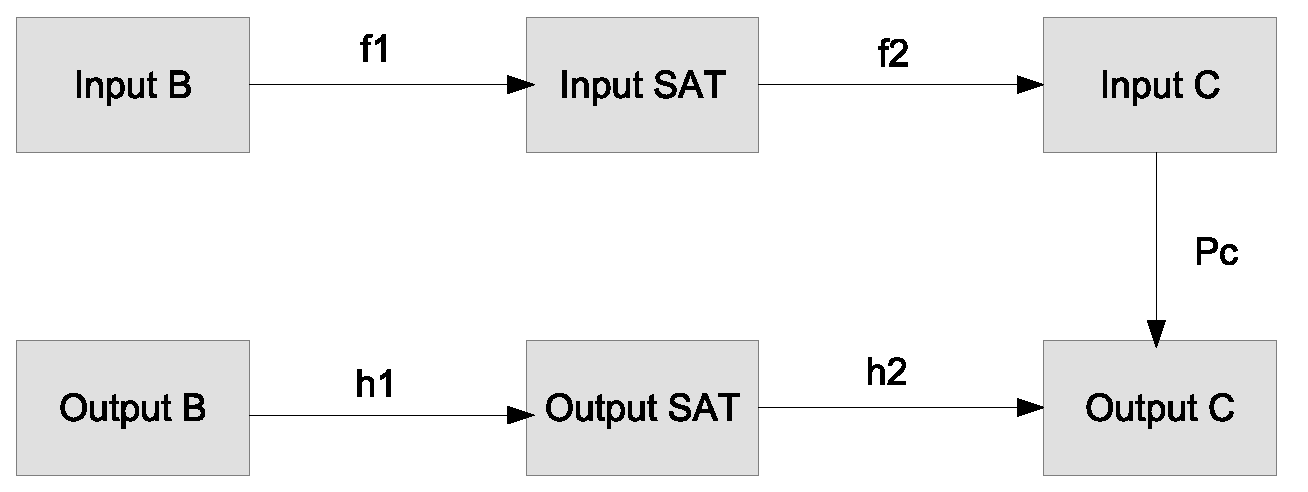
\includegraphics[width=4.0in]{figures/SATC}
\caption{\label{fig:relation-npc}Relations of NPC}
\end{center}
\end{figure}

NP-hard: problems cannot verify in polynomial time.

\section{SAT}
Then we talk about SAT problems. SAT is the problem of determining if there exists an interpretation that satisfies a given Boolean formula.
2SAT is not a NPC problem, but 3SAT is a NPC problem.
Then we want to verify that SAT $rightarrow$ 3SAT. The reduction process can be seen in Figure~\ref{fig:reduction-sat}

\begin{figure}[bht]
\begin{center}
     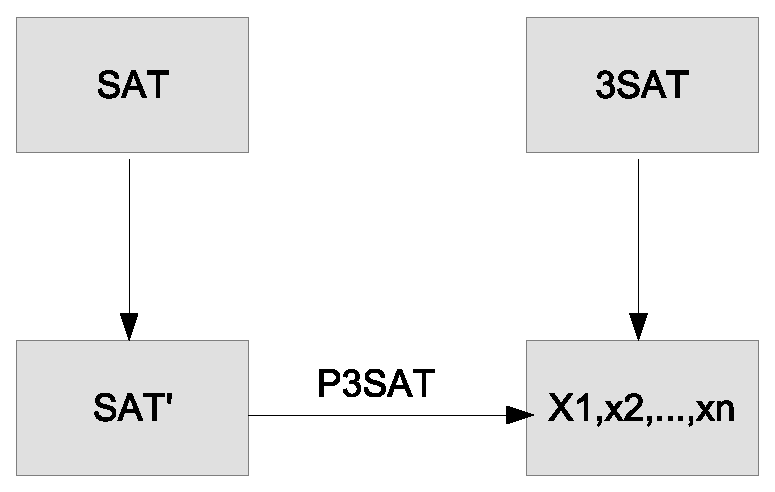
\includegraphics[width=3.0in]{figures/reduction-sat}
\caption{\label{fig:reduction-sat}reduction of SAT and 3SAT}
\end{center}
\end{figure}

Suppose we have a SAT problem $X_1 \vee X_2\vee X_3 \vee X_4\vee X_5\vee X_6$, then we transform it to 
$(X_1 \vee X_2 \vee y_1) \wedge (\overline{y_1} \vee X_3 \vee y_2) \wedge (\overline{y_2} \vee X_4 \vee y_3) \wedge (\overline{y_3} \vee X_5 \vee x_6)$ 

Then we want to verify two condistions:
\begin{enumerate}
	\item If ${x}$ is a solution of SAT version, then ${x,y}$ is a solution of 3SAT version.
	\item If ${x}$ is not a solution of SAT version, then ${x,y}$ is not a solution of 3SAT version.
\end{enumerate}

For first condition, if ${x}$ is a solution of SAT version, then one of ${x}$ is true. Assume $x_1$ is true, we make all of the ${y}$ to be false, then 3SAT version is true. 
So we can get the condition one to be true.

For second condition, if ${x}$ is not a solution of SAT version, then all of the ${x}$ are false. So not matter what ${y}$ is, 3SAT version is always false. So we can get the condition two to be true
\end{document}
